%!TEX root = ../../main.tex

\toggletrue{image}
\toggletrue{imagehover}
\chapterimage{moving}
\chapterimagetitle{\uppercase{Moving}}
\chapterimageurl{https://xkcd.com/466/}
\chapterimagehover{We need a special holiday to honor the countless kind souls with unsecured networks named 'linksys'.}

\chapter{Computernetzwerke}
\label{chapter-netzwerke}

Sie sind vermutlich bereits Teil eines Netzwerks. Damit ist nicht Ihr Account bei einer sozialen Plattform, wie z.B. Instagram, gemeint, sondern ein Computernetzwerk. Sobald Sie ein Notebook, einen Desktop-Computer oder ein Smartphone besitzen, sind Sie vermutlich automatisch mit dem \ac{WLAN} verbunden und somit Teil des Internets. In diesem Kapitel klären wir, was ein Computernetzwerk ist und wie das Internet aufgebaut ist. Die Lernziele lauten:

\newcommand{\netzwerkeLernziele}{
\protect\begin{todolist}
\item Sie erklären, was ein Computernetzwerk ist und geben ein Beispiel.
\item Sie erklären, was das Internet ist.
\item Sie erklären, wie ein Computer Zugang zum Internet erhält.
\end{todolist}
}

\lernziel{\autoref{chapter-netzwerke}, \nameref{chapter-netzwerke}}{\protect\netzwerkeLernziele}

\netzwerkeLernziele

\section{Was ist ein Computernetzwerk?}

\autoref{figure-network-pc-router} zeigt ein Beispiel für ein drahtloses lokales Netzwerk (eng. \ac{WLAN}). Alle Computer sind über den Router mit dem \ac{WLAN} verbunden. Der Router ist ein elektronisches Gerät und sorgt dafür, dass die Computer miteinander verbunden werden und im Netzwerk für den Datenaustausch erreichbar sind.

\begin{figure}[htb]
\begin{minipage}{0.5\textwidth	}
\centering
\begin{tikzpicture}
  \pic(comp0) [
    draw,
    fill = gray!30,
    pic text = {PC},
    scale=0.1
  ] at (-2,0)
  {computer};
  \node at ([yshift=.25cm]comp0-m.north) {\faWifi};
  \pic(comp1) [
    draw,
    fill = gray!30,
    pic text = {PC},
    scale=0.1
  ] at (2,0)
  {computer};
  \node at ([yshift=.25cm]comp1-m.north) {\faWifi};
  \pic(comp2) [
    draw,
    fill = gray!30,
    pic text = {PC},
    scale=0.1
  ] at (-1,1.6)
  {computer};
  \node at ([yshift=.25cm]comp2-m.north) {\faWifi};
  \pic(comp3) [
    draw,
    fill = gray!30,
    pic text = {PC},
    scale=0.1
  ] at (1,1.6)
  {computer};
  \node at ([yshift=.25cm]comp3-m.north) {\faWifi};
  \node[scale=0.2] (router) at (0,0) {\router{}};
  \node at ([yshift=.25cm]router.north) {\faBroadcastTower};
\end{tikzpicture}
\caption{Das Symbol in der Mitte repräsentiert einen Router (siehe \autoref{figure-fritzbox}).}
\label{figure-network-pc-router}
\end{minipage}
\hfill
% https://m.media-amazon.com/images/I/71kwiZApINL._AC_SX450_.jpg
\begin{minipage}{0.45\textwidth}
\centering
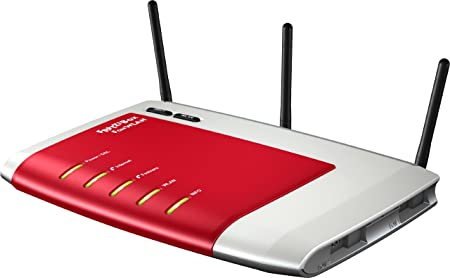
\includegraphics[scale=0.3]{fritzbox}
\caption{Handelsüblicher Router für den Heimgebrauch.}
\label{figure-fritzbox}
\end{minipage}
\end{figure}

\begin{definition}[Computernetzwerk]
Eine Menge von unabhängigen Computern (unterschiedliche Hardware, Betriebssysteme, \dots), die durch eine Technologie (zum Beispiel \ac{WLAN}) miteinander verbunden sind und Daten austauschen.
\end{definition}

Wir verwenden die Begriffe Computernetzwerk (eng. computer network) und Netzwerk von nun an als Synonym, da wir uns hier nur mit Computernetzwerken beschäftigen. Computer können sich auch mit einem Kabel über einen Router oder Switch verbinden und ein Netzwerk aufbauen. Wir sprechen dann von einem \ac{LAN}.

\begin{important}
  Für ein Netzwerk ist der Zugang zum Internet nicht notwendig. Der Router kann auch \say{nur} eingesetzt werden, um ein Netzwerk aufzubauen und Daten auszutauschen.
\end{important}

\section{Was ist das Internet?}

% https://norbert-pohlmann.com/app/uploads/2017/07/165-Netz-Deutschland-Zahl-autonomer-Systeme-wächst-stetig-Prof.-Norbert-Pohlmann.pdf

Das Internet ist eine Kurzform für \textbf{Inter}connected \textbf{Net}work. Es stellt einen Verbund von Netzwerken dar und ermöglicht den Datenaustausch zwischen Computern aus unterschiedlichen Netzwerken.

\begin{definition}[Internet]
Das weltweite Internet ist ein Zusammenschluss von unabhängigen Netzwerken. Es ist ein Netzwerk von Netzwerken und steht der Allgemeinheit zur Verfügung.
\end{definition}

\autoref{figure-internet} zeigt die Idee des Internets. Lokale Netzwerke (wie z.B. das Netzwerk von Alice) besitzen einen Router. Diese Router stellen eine Verbindung zum \ac{ISP} her. Dies geschieht in der Regel durch ein Kupfer- oder Glasfaserkabel. Dadurch erhalten Haushalte Zugang zum Internet. In der Schweiz sind die Swisscom oder UPC bekannte \ac{ISP} (oft auch einfach nur Provider genannt). Der Zugang zum Internet ist eine kostenpflichtige Dienstleistung.

\begin{figure}[htb]
\centering
\begin{adjustbox}{width=0.7\textwidth}
\begin{tikzpicture}
\begin{scope}[on background layer]
\node[cloud, draw=black, dashed, minimum width = 1.1\textwidth, minimum height = 10cm] (internet) at (2,1.75) {};
\end{scope}
\node[cloud, fill = gray!10, minimum width = 10cm, minimum height = 5cm] (network1) at (0,0) {};
\node[cloud, fill = gray!20, minimum width = 5cm, minimum height = 6cm] (network2) at (7,2) {};
\node[cloud, fill = gray!30, minimum width = 8cm, minimum height = 4cm] (network3) at (-1,3) {};
\node[scale=0.2] (router1) at (0,0) {\router{}};
\node (isp) at (0,0.5) {\acs{ISP}};
\node[scale=0.2] (router2) at (2,2) {\router{}};
\node (isp) at (2.5,2.5) {\acs{ISP}};
\node[scale=0.2] (router3) at (4,3) {\router{}};
\node (isp) at (4,3.5) {\acs{ISP}};
\draw (router1) edge[very thick, darkgray!30!gray] (router2);
\draw (router2) edge[very thick, darkgray!30!gray] (router3);
\node[my cloud, font=\small] (bob) at (3, 0) {Bobs Hütte} edge[very thick, darkgray!30!gray] (router1);
\node[my cloud, font=\small] (alice) at (-3, 0) {Haus von Alice} edge[very thick, darkgray!30!gray] (router1);
\node[my cloud, font=\small] (carol) at (-3, 3) {Carols Versteck} edge[very thick, darkgray!30!gray] (router2);
\node[my cloud, font=\small] (oscar) at (1, 4) {Oscars Wohnung} edge[very thick, darkgray!30!gray] (router2);
\node[my cloud, font=\small] (trent) at (7, 3) {Trents Palast} edge[very thick, darkgray!30!gray] (router3);
\node[my cloud, font=\small] (eve) at (7, 0.5) {Eves Hotel} edge[very thick, darkgray!30!gray] (router3);
\end{tikzpicture}
\end{adjustbox}
\caption{Schematische Darstellung des Internets. Die gestrichelte Wolke stellt das Internet als Zusammenschluss von mehreren Netzwerken (graue Wolken) dar.}
\label{figure-internet}
\end{figure}

\begin{figure}[htb]
\centering
\begin{minipage}{0.6\textwidth}
Die Netzwerke der Provider sind wieder miteinander verbunden. Hier kommen keine haushaltsüblichen Router, sondern Hochleistungssysteme, die Daten effizient zwischen Netzwerken bewegen, zum Einsatz. Die Netzwerke werden mit Kabel an den Router angeschlossen und der Router sorgt für hohe Datenübertragungsraten (mehrere Terabits pro Sekunde). \autoref{figure-router-cisco} zeigt mehrere Hochleistungsrouter. Auch ein lokaler Provider (wie z.B. die Swisscom) muss in der Regel mit einem globalen Provider einen Vertrag zur Nutzung der Netzwerke abschliessen. Die globalen \ac{ISP} sorgen für den Verbund der globalen Netzwerke, das heisst auch interkontinental durch zum Beispiel Unterseekabel.
\end{minipage}
\hfill
\begin{minipage}{0.35\textwidth}
\centering
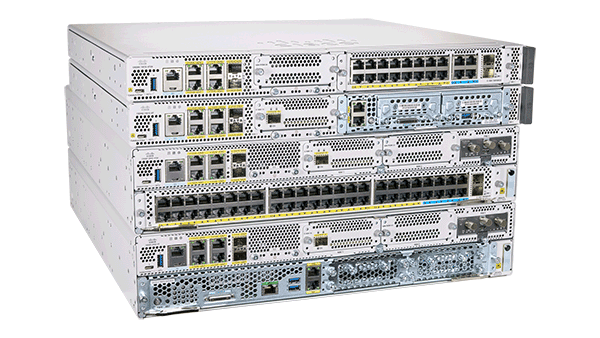
\includegraphics[scale=0.25]{cisco_router}
\caption{Mehrere Router mit mehreren Netzwerkanschlüssen der Firma CISCO.}
\label{figure-router-cisco}
% https://www.cisco.com/c/de_ch/products/routers/index/jcr:content/Grid/raw_html_wrapper_f28/parsys_content/category_atl_copy_co/layout-category-atl/blade_7bfa/bladeContents/scroll_container_223/scrollContent/tile_b661.img.png/1616053511233.png
\end{minipage}
\end{figure}